\documentclass[10pt]{beamer}

% Beamer style
%\usetheme[secheader]{Madrid}
% \usetheme{CambridgeUS}
\useoutertheme{infolines}
\usecolortheme[rgb={0.65,0.15,0.25}]{structure}
% \usefonttheme[onlymath]{serif}
\beamertemplatenavigationsymbolsempty
%\AtBeginSubsection

% Packages
%\usepackage[french]{babel}
\usepackage[latin1]{inputenc}
\usepackage{color}
\usepackage{xspace}
%\usepackage{dsfont, stmaryrd}
\usepackage{amsmath, amsfonts, amssymb}
\usepackage{epsfig}
\usepackage{url}
\usepackage{/home/robin/LATEX/Biblio/astats}
%\usepackage[all]{xy}
\usepackage{graphicx}

% Commands
\definecolor{darkred}{rgb}{0.65,0.15,0.25}
%\newcommand{\emphase}[1]{\textcolor{darkred}{#1}}
\newcommand{\emphase}[1]{{#1}}
\newcommand{\paragraph}[1]{\textcolor{darkred}{#1}}
\newcommand{\refer}[1]{{\footnotesize{\textcolor{gray}{{\cite{#1}}}}}}
\newcommand{\Refer}[1]{{\footnotesize{\textcolor{gray}{{#1}}}}}
\renewcommand{\newblock}{}

% Symbols
\newcommand{\dd}{\xspace\text{d}}
\newcommand{\Esp}{\mathbb{E}}
\newcommand{\Ibb}{\mathbb{I}}
\newcommand{\Cov}{\mathbb{C}\text{ov}}
\newcommand{\Var}{\mathbb{V}}
\newcommand{\Mcal}{\mathcal{M}}
\newcommand{\Ncal}{\mathcal{N}}
\newcommand{\pa}{\text{pa}}
\newcommand{\ra}{\emphase{\mathversion{bold}{$\rightarrow$}~}}
\newcommand{\Scal}{\mathcal{S}}

% Directory
\newcommand{\figmixt}{/home/robin/ENSEIGN/COURS/MELANGE}
\newcommand{\figbma}{/home/robin/RECHERCHE/RUPTURES/MELANGE/Exemples/Grippe}
\newcommand{\fignet}{../FIGURES}
\newcommand{\figeco}{/home/robin/RECHERCHE/ECOLOGIE/EXPOSES/FIGURES}
%\newcommand{\figmotif}{/home/robin/RECHERCHE/RESEAUX/Motifs/FIGURES}


%====================================================================
%====================================================================

%====================================================================
%====================================================================
\begin{document}
%====================================================================
%====================================================================

%====================================================================
\title[Looking for adaptive shifts]{Unsupervised classification of species: Looking for adaptive shifts in evolution}

\author[S. Robin]{P. Bastide, M. Mariadassou, \underline{S. Robin}}

\institute[INRA / AgroParisTech]{INRA / AgroParisTech \\
%  \vspace{-.1\textwidth}
  \begin{tabular}{ccccc}
    
\includegraphics[height=.08\textheight]{\fignet/LogoINRA-Couleur} & 
    \hspace{.02\textheight} &
    
\includegraphics[height=.08\textheight]{\fignet/logagroptechsolo} & 
    \hspace{.02\textheight} &
    
\includegraphics[height=.09\textheight]{\fignet/logo-ssb}
    \\ 
  \end{tabular} \\
  \bigskip
  }

\date[WGMBC, Seattle, 2015]{WGMBC, July 2015, Seattle}

%====================================================================
%====================================================================
\maketitle
%====================================================================

%====================================================================
%====================================================================
\section{Modeling adaptive shifts}
% \frame{\frametitle{Outline} \tableofcontents[currentsection]}
%====================================================================
\frame{\frametitle{Diversity of a trait}

  The diversity of a trait among a set of species results from:
  \begin{itemize}
   \item their shared history,
   \item potential isolated shifts corresponding to adaptive shifts due, e.g. to changes of ecological niche.
  \end{itemize}
  $$
  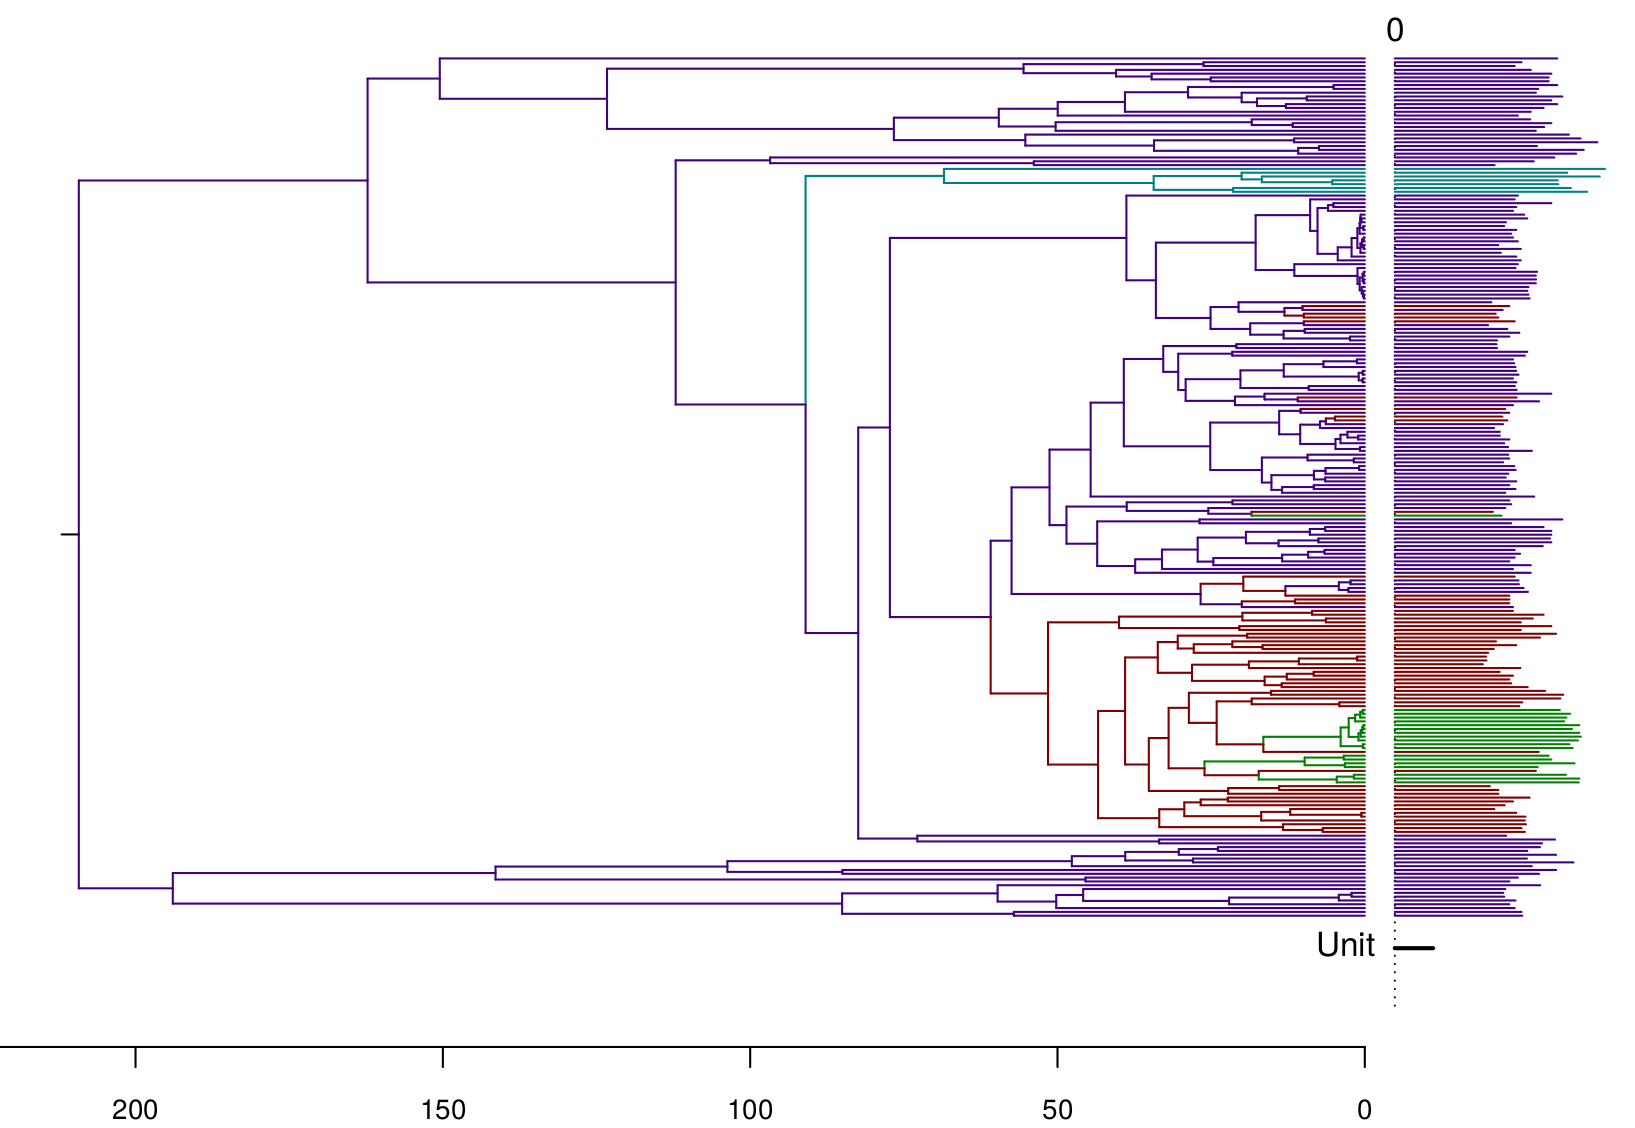
\includegraphics[width=.6\textwidth, clip=]{../FIGURES/plot_data_chel-intro-SR}
  $$
  \refer{JSA11}
  }

%====================================================================
\frame{\frametitle{Evolution of a trait}

  \begin{tabular}{cc}
    \begin{tabular}{p{.5\textwidth}}	
    Phylogenetic tree \\
    \vspace{-.15\textheight}
    \includegraphics[width=.5\textwidth, clip=]{../FIGURES/plot_tree_tims_2-1}
    \\
    \vspace{-.1\textheight}
    Process on the tree  \\
    \vspace{-.15\textheight}
    \includegraphics[width=.5\textwidth, clip=]{../FIGURES/plot_BM_sim_2-1}
    \end{tabular}
    &    
    \hspace{-.1\textwidth}
    \begin{tabular}{p{.45\textwidth}}
    \paragraph{Model for trait $X$:} no cluster\\ ~
    \begin{itemize}
    \item $X$ is a random process (e.g. Brownian motion = BM) that goes along the
    branches of the tree \refer{Fel85}; \\ ~
    \item at each internal nodes, independent copies of the processes bifurcate; \\ ~
    \item only the leafs $Y_1, Y_2, \dots Y_n$ are observed: 
    \begin{eqnarray*}
    \text{for BM:} \quad 
    \Var(X_A|R) & = & \sigma^2 t, \\
    \Cov(X_A, X_B|R) & = & \sigma^2 t_{AB},
    \end{eqnarray*}
    \end{itemize} \\
  \end{tabular}
  \end{tabular}
  }

%====================================================================
\frame{\frametitle{Introducing shifts}

  \begin{tabular}{cc}
    \begin{tabular}{p{.5\textwidth}}	
    Phylogenetic tree \\
    \vspace{-.15\textheight}
    \includegraphics[width=.5\textwidth, clip=]{../FIGURES/plot_tree_tims_shift-1}
    \\
    \vspace{-.1\textheight}
    Process on the tree  \\
    \vspace{-.15\textheight}
    \includegraphics[width=.5\textwidth, clip=]{../FIGURES/plot_BM_sim_shit-1} \\
    clusters: $(A, B, D)$ / $(C, E)$
    \end{tabular}
    &    
    \hspace{-.1\textwidth}
    \begin{tabular}{p{.45\textwidth}}
    \paragraph{Model with $K$ shifts:} clusters\\ ~
    \begin{itemize}
    \item Same model as before; \\ ~
    \item at the start of $K$ branches $\tau_k$, shifts (with magnitude $\delta_k$;) occur; \\ ~
    \item the distribution of the process is shifted accordingly: \\
    for BM
    \begin{eqnarray*}
    \mu_j & = & \mu_{\pa(j)} + \sum_k \delta_k \mathbb{I}\{\tau_k=b_j\},
    \end{eqnarray*}
    \end{itemize} \\
  \end{tabular}
  \end{tabular}
}

%====================================================================
%====================================================================
\section{Inference}
%====================================================================

%====================================================================
\frame{\frametitle{Incomplete data model perspective}

%   \hspace{-.05\textwidth}
  \begin{tabular}{cc}
    \begin{tabular}{p{.5\textwidth}}
	 \paragraph{Complete data} $X = (Z, Y)$
	 \begin{itemize}
	  \item $(Z_i) = $ traits at the internal nodes (ancestors);
	  \item $(Y_j) = $ traits at the leafs (extant species).
	 \end{itemize}
    \end{tabular}
    & 
    \hspace{-.1\textwidth}
    \begin{tabular}{p{.5\textwidth}}
      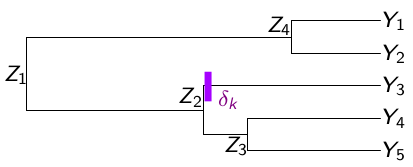
\includegraphics[width=.45\textwidth]{../FIGURES/IncompleteData-BMR15}
    \end{tabular}
  \end{tabular}

  \bigskip \pause
  \paragraph{EM algorithm.}
  \begin{itemize}
   \item E-step: via upward-downward recursion; %\\
%    (or direct conditional multivariate distribution $p(Z|Y)$);
   \item M-step: for BM, $\displaystyle{X_j|X_{\pa(j)} \sim \Ncal(X_{\pa(j)}+ \sum_k \delta_k \mathbb{I}\{\tau_k=b_j\}, \ell_j \sigma^2)}$, and
   \begin{eqnarray*}
    \Esp \log p(X) & = & \sum_j \Esp \log p(X_j | X_{\pa(j)})
   \end{eqnarray*}
   \ra the optimal allocation of the shifts to the branches is trivial;
   \item Intialization: using Lasso (see next).
  \end{itemize}

  }

%====================================================================
\frame{\frametitle{Regression perspective}

  \begin{tabular}{cc}
    \begin{tabular}{p{.5\textwidth}}
	 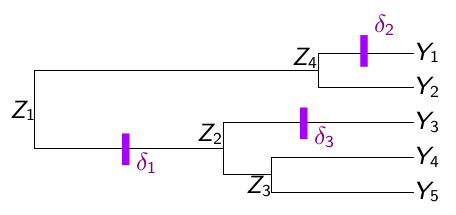
\includegraphics[width=.5\textwidth]{../FIGURES/RegressionView-BMR15}
    \end{tabular}
    & 
    \hspace{-.1\textwidth}
    \begin{tabular}{p{.5\textwidth}}
    {\scriptsize
    \[
    \Delta = \begin{pmatrix}
	 \mu\\ \delta_1\\ 0\\  0\\ \delta_2\\ 0\\ \delta_3\\ 0\\ 0\\
    \end{pmatrix}                           
    \qquad 
    T \Delta = \begin{pmatrix}
	 \mu + \delta_2\\ \mu\\ \mu + \delta_1 + \delta_3\\ \mu + \delta_1\\ \mu + \delta_1\\ 
    \end{pmatrix}
    \]
    }
    \end{tabular} 
    \\
    \begin{tabular}{p{.5\textwidth}}
         {\scriptsize
         \[
         \!\!\!T\!=\!
         \bordermatrix{
         \!&Z_1\!\!\!&Z_2\!\!\!&Z_3\!\!\!&Z_4\!\!\!&\!\!\!&Y_1\!\!\!&Y_2\!\!\!&Y_3\
         \!\!&Y_4\!\!\!&Y_5\cr
         Y_1\!&1&0&0&1&\!\!\!&1&0&0&0&0 \cr
         Y_2\!&1&0&0&1&\!\!\!&0&1&0&0&0 \cr
         Y_3\!&1&1&0&0&\!\!\!&0&0&1&0&0 \cr
         Y_4\!&1&1&1&0&\!\!\!&0&0&0&1&0 \cr
         Y_5\!&1&1&1&0&\!\!\!&0&0&0&0&1 \cr 
         }\]
         }
    \end{tabular}
    & 
    \hspace{-.1\textwidth}
    \begin{tabular}{p{.5\textwidth}}
    \begin{eqnarray*}
    \text{for BM:} \quad Y & = & T\Delta + E \\
    E  & \sim & \Ncal(0, \Sigma)
    \end{eqnarray*}
    \end{tabular}
  \end{tabular}

  \begin{itemize}
   \item Initialization: $\arg\min_\delta \|Y - T\Delta\|^2_{\Sigma^{-1}} + \lambda |\Delta|$;
   \item Identifiability issues: the null space of $T$ does not reduce to $0$;
   \item Useful representation for model selection.
  \end{itemize}
  }

%====================================================================
%====================================================================
\section{Identifiability}
%====================================================================
\frame{\frametitle{Identifiability}

  \begin{itemize}
   \item Shift allocation results in a coloring of the leafs (only observable);
   \item Different scenarios may results in the same coloring;
   \item Some scenarios are parsimonious, some are not.
  \end{itemize}
  
  \begin{overprint}
   \onslide<1>
     \begin{tabular}{p{.25\textwidth}p{.05\textwidth}p{.25\textwidth}p{.05\textwidth}p{.25\textwidth}}
	 \begin{tabular}{c}
	 \includegraphics[width=0.15\textwidth]{../FIGURES/colours_1_nodes_gray} \\
	 2 colors \\ ~
	 \end{tabular}
	 & 
	 \begin{tabular}{c}
	 $:$
	 \end{tabular}
	 & 
	 \begin{tabular}{c}
	 \includegraphics[width=0.15\textwidth]{../FIGURES/colours_2_nodes_gray} \\
	 non \\
	 parsimonious
	 \end{tabular}
	 & 
	 \begin{tabular}{c}
	 $<$
	 \end{tabular}
	 & 
	 \begin{tabular}{c}
	 \includegraphics[width=0.15\textwidth]{../FIGURES/colours_3_nodes_gray} \\
	 parsimonious \\ ~
	\end{tabular}
  \end{tabular}
  \onslide<2>
     \begin{tabular}{p{.25\textwidth}p{.05\textwidth}p{.25\textwidth}p{.05\textwidth}p{.25\textwidth}}
	 \begin{tabular}{c}
	 \includegraphics[width=0.15\textwidth]{../FIGURES/colours_bis_1_nodes_gray} \\
	 3 colors
	 \end{tabular}
	 & 
	 \begin{tabular}{c}
	 $:$
	 \end{tabular}
	 & 
	 \begin{tabular}{c}
	 \includegraphics[width=0.15\textwidth]{../FIGURES/colours_bis_2_nodes_gray} \\
	 parsimonious
	 \end{tabular}
	 & 
	 \begin{tabular}{c}
	 $\sim$
	 \end{tabular}
	 & 
	 \begin{tabular}{c}
	 \includegraphics[width=0.15\textwidth]{../FIGURES/colours_bis_3_nodes_gray} \\
	 parsimonious
	\end{tabular}
  \end{tabular}
  \end{overprint}
}

%====================================================================
\frame{ \frametitle{Number of models with $K$ shifts}

  \paragraph{No homoplasy:} 1 shift = 1 new color.
  $$
  K \text{ shifts} \quad \Leftrightarrow \quad K + 1 \text{ colors}
  $$
 
  \bigskip
  \paragraph{Actual number of models:}
  \begin{align*}
  \Scal_K^{PI} &= \Scal_K^{P}/\sim; \\
  \Scal_K^P & = \{\text{Parsimonious allocations of $K$ shifts}\} %\\
%   \Scal_K^{PI} & \simeq \{\text{Tree compatible coloring of tips in $K+1$ colors}\} 
  \end{align*}
  \ra Complexity of the $K$-shifts model class $= \# \Scal_K^{PI}$ ?

  \bigskip \pause
  \paragraph{Contribution:}
  \begin{itemize}
  \item $\#{\Scal_K^{PI}} \leq \binom{m+n-1}{K}$
  \item $\#{\Scal_K^{PI}}$ depends on the topology of the tree and can be computed recursively.
  \item For a binary tree: $\#{\Scal_K^{PI}} = \binom{2n-2-K}{K}$.
  \item Parsimonious equivalent scenarios can be enumerated (generalization of \refer{Fel04}.)
  \end{itemize}
}

%====================================================================
\frame{ \frametitle{Example of equivalent scenarios}

  OU (see next) model: this 5 configurations only count for 1.
  $$
  \includegraphics[width=.8\textwidth]{../FIGURES/plot_parsimony-1}
  $$
}

%====================================================================
\frame{ \frametitle{Model selection: $K =$?}

  \paragraph{Specificity:} due to the discrete nature of the shift location, standard criteria (AIC, BIC) do not apply.
  
  \bigskip \bigskip \pause
  \paragraph{Penalized criterion.} Under the BM model $Y = T \Delta + E, \qquad E \sim \Ncal(0, \Sigma)$, taking
  $$
  \widehat{\eta} = \arg\min_{\eta \in \Mcal} \|Y - \widehat{s}_\eta\|^2_{\Sigma^{-1}} + (1 + \text{Pen}(K_\eta))
  $$
  where
  $$
  \Mcal = \bigcup_{K \geq 0} \Scal^{PI}_K, 
  \qquad
  \text{Pen}(K) = f(n, K, \# \Scal^{PI}_K)
  $$
  ensures the oracle inequality
  $$
  \|Y - \widehat{s}_\eta\|^2_{\Sigma^{-1}}
  \leq C_1 \left(\inf_{\eta \in \Mcal} \|s - \widehat{s}_\eta\|^2_{\Sigma^{-1}} + C_2(n, \eta) + C_3(n) \right)
  $$
  
  \paragraph{Proof.} Adaptation of \refer{BGH09}. 
}

%====================================================================
%====================================================================
\section{Illustration}
%====================================================================

%====================================================================
\frame{\frametitle{Brownian motion vs Ornstein-Uhlenbeck process}

  \bigskip
  \paragraph{Brownian motion:} $\dd X(t) = \sigma \dd B(t)$ \refer{Han97} 
  \begin{itemize}
   \item Easy to handle (no memory);
   \item Not realistic: no stationary distribution \ra the trait can wander anywhere.
  \end{itemize}

  \bigskip \pause
  \paragraph{Ornstein-Uhlenbeck:} $\dd X(t) = \sigma \dd B(t) - \alpha \left(X(t) - \beta\right) \dd t$ \refer{BuK04}
  \begin{itemize}
   \item Continuous counterpart of an $AR(1)$ time series;
   \item Recall with strength $\alpha$ toward an 'optimum' $\beta$;
   \item More realistic: has stationary distribution $\Ncal(\beta, \sigma^2/2\alpha)$;
   \item Here: shifts occur in $\beta$. \\
   \begin{flushright}
   \vspace{-.15\textheight}
   \includegraphics[width=.5\textwidth]{../FIGURES/plot_OU_sim_shit-1}
   \end{flushright}
  \end{itemize} 

  \vspace{-.05\textheight}
  \ra Everything works (almost) the same as for BM ... in a more intricate way.
  }

%====================================================================
\frame{ \frametitle{Chelonia turtles}

  \only<1>{
\begin{columns}
\begin{column}{0.55\textwidth}
\begin{minipage}[c][\textheight][c]{\linewidth}
\vskip -1 cm
    \includegraphics[width=\linewidth]{../FIGURES/plot_chel_data1-1} \\
    {\footnotesize Colors: habitats.\\ Boxes: selected EM regimes.}
\end{minipage}
\end{column}
\begin{column}{0.45\textwidth}
\begin{minipage}[t][.6\textheight][c]{\linewidth}
\end{minipage}
\end{column}
\end{columns}
}
\only<2>{
\begin{columns}
\begin{column}{0.55\textwidth}
\begin{minipage}[c][\textheight][c]{\linewidth}
\vskip -1 cm
    \includegraphics[width=\linewidth]{../FIGURES/plot_chel_data-1} \\
    {\footnotesize Colors: habitats.\\ Boxes: selected EM regimes.}
\end{minipage}
\end{column}
\begin{column}{0.45\textwidth}
\begin{minipage}[t][.6\textheight][c]{\linewidth}
\vskip - 4 cm
\includegraphics[width=0.5\textwidth]{../FIGURES/Chelonia_mydas.jpg} \\
{\footnotesize Chelonia mydas}
\end{minipage}
\end{column}
\end{columns}
}
\only<3>{
\begin{columns}
\begin{column}{0.55\textwidth}
\begin{minipage}[c][\textheight][c]{\linewidth}
\vskip -1 cm
\includegraphics[width=\linewidth]{../FIGURES/plot_chel_data3-1}  \\
{\footnotesize Colors: habitats.\\ Boxes: selected EM regimes.}
\end{minipage}
\end{column}
\begin{column}{0.45\textwidth}
\begin{minipage}[t][.6\textheight][c]{\linewidth}
\includegraphics[width=0.5\textwidth]{../FIGURES/Geochelone_nigra_abingdoni.jpg} \\
{\footnotesize Geochelone nigra abingdoni}
\end{minipage}
\end{column}
\end{columns}
}
\only<4>{
\begin{columns}
\begin{column}{0.55\textwidth}
\begin{minipage}[c][\textheight][c]{\linewidth}
\vskip -1 cm
\includegraphics[width=\linewidth]{../FIGURES/plot_chel_data5-1} \\
{\footnotesize Colors: habitats.\\ Boxes: selected EM regimes.}
\end{minipage}
\end{column}
\begin{column}{0.45\textwidth}
\begin{minipage}[t][.6\textheight][c]{\linewidth}
\vskip - 4 cm
\includegraphics[width=0.5\textwidth]{../FIGURES/Dudhwalive_chitra.jpg} \\
{\footnotesize Chitra indica}
\end{minipage}
\end{column}
\end{columns}
}
\only<5>{
\begin{columns}
\begin{column}{0.55\textwidth}
\begin{minipage}[c][\textheight][c]{\linewidth}
\vskip -1 cm
\hspace{.025\textwidth}
\includegraphics[width=\linewidth]{../FIGURES/plot_chel_data4-1} \\
{\footnotesize Colors: habitats.\\ Boxes: selected EM regimes.}
\end{minipage}
\end{column}
\begin{column}{0.5\textwidth}
\begin{minipage}[t][.6\textheight][c]{\linewidth}
\vskip - 3 cm
{\footnotesize
\begin{table}[!ht]
\begin{center}
\begin{tabular}{l|c|c}
\hline
  & Habitat & EM\\ \hline
Nb shifts & 16 & 5\\ \hline
Nb regimes & 4 & 6\\ \hline
$\log P$ & -135.56 & -97.59\\ \hline
$\ln 2 / \alpha$ (\%) & 7.83 & 5.43\\ \hline
$\gamma^2$ & 0.35 & 0.22\\ \hline
CPU (mn) & 1.25 & 134.49\\ \hline
\end{tabular}
\end{center}
\end{table}
}
\end{minipage}
\end{column}
\end{columns}
}
}

%====================================================================
\frame{\frametitle{Conclusion \& Future works}

  \paragraph{Conclusions.}
  \begin{itemize}
   \item Comprehensive estimation framework: EM algorithm + identifiability + model selection;
   \item Code available at \url{https://github.com/pbastide/Phylogenetic-EM}.
  \end{itemize}

  \bigskip \bigskip
  \paragraph{Future work.}
  \begin{itemize}
   \item Estimating $\alpha$ in the OU model;
   \item Multivariate traits; 
   \item Deal with the uncertainty of the tree;
   \item Use fossil records (which would be most useful to distinguish between equivalent scenarios).
  \end{itemize}

}

%====================================================================
\frame[allowframebreaks]{ \frametitle{References}
{\footnotesize
  \bibliography{/home/robin/Biblio/BibGene}
  \bibliographystyle{/home/robin/LATEX/Biblio/astats}
  %\bibliographystyle{plain}
  }
}

%====================================================================
\frame{\frametitle{Notations}
  
  $$
  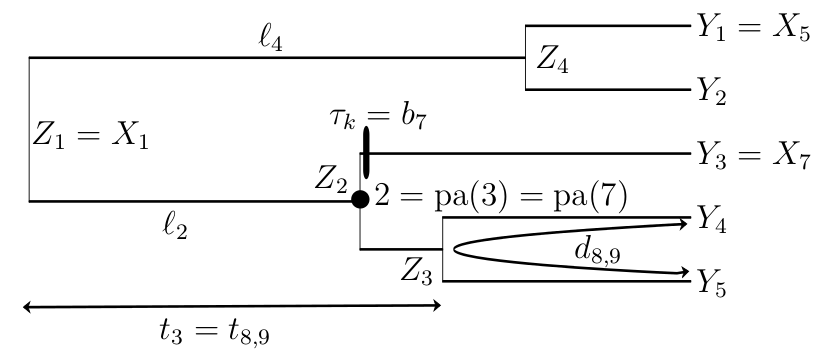
\includegraphics[width=.8\textwidth]{../FIGURES/Notations-BMR15}
  $$
  
  }

%====================================================================
%====================================================================
\end{document}
%====================================================================
%====================================================================

  \begin{tabular}{cc}
    \begin{tabular}{p{.5\textwidth}}
    \end{tabular}
    & 
    \hspace{-.02\textwidth}
    \begin{tabular}{p{.5\textwidth}}
    \end{tabular}
  \end{tabular}

